\documentclass[11pt,notes]{beamer}
\usetheme{Boadilla}

%\usepackage{pgfpages}
\usepackage[utf8]{inputenc}
\usepackage[T1]{fontenc}
\usepackage{graphicx}
\usepackage{bbding}
\usepackage{ textcomp }
\usepackage{color}
\usepackage{pgf}
\usepackage{tikz}
\usetikzlibrary{arrows,automata,positioning}

\setbeamertemplate{caption}[]

\newcommand*\tick{\item[\Checkmark]}
\newcommand*\fail{\item[\XSolidBrush]}
\newcommand*\prog{\item[\textgreater]}
\newcommand*\fstar{\item[\FiveStar]}

\author{Simon Schlepphorst, Federico Diaz Capriles}
\title{Ising Model}
\subtitle{A Statistical System at Finite Temperature}

\logo{
\includegraphics[height=1.5cm]{Images/logo}\vspace{220pt}}

\institute{Uni Bonn}

\date{16 March 2017}

\setbeamercovered{transparent}

\setbeamertemplate{navigation symbols}{}









\begin{document}
	

\begin{frame}
	\titlepage
\end{frame}

\begin{frame}
	\tableofcontents
\end{frame}

\section{Introduction}
\subsection{Theory}
\begin{frame}
	\frametitle{Introduction}
	\framesubtitle{Theory}
	\begin{minipage}{.6\textwidth}
			\begin{center}
			
\begin{tikzpicture}
				\draw[step=.5cm,gray,very thin] (0.1,0.1) grid (2.9,2.9);
				\fill[black] (0.1,0.1) rectangle (.5,1.5);
				\fill[black] (0.1,1.5) rectangle (2,2);
				\fill[black] (2,0.1) rectangle (2.5,0.5);
				\fill[black] (1.5,0.5) rectangle (2,1);
				\fill[black] (0.5,1) rectangle (1,1.5);
				\fill[black] (2,2) rectangle (2.9,2.9);
			\end{tikzpicture}
		\end{center}
	\end{minipage}%
	\begin{minipage}[]{.4\textwidth}
		$ \square $ Spin up \\ 
		$ \blacksquare $ Spin down 
	\end{minipage}
	\vspace{-.05cm}
	\begin{equation}
		 \mathcal{H}(\textbf{s}) = -J \sum_{\langle i, j \rangle} s_{i} s_{j}
	\end{equation}
	{\scriptsize \begin{equation*}
		 s_{n} \in \{-1,+1\}
	\end{equation*}}\vspace{-.5cm}
	\begin{equation}
		\textbf{s} = (s_{1}, s_{2}, \dots, s_{N})
	\end{equation}
	\begin{equation}
		\mathcal{Z} = \sum_{\textbf{s}} exp(-\frac{1}{k_{B} T}\mathcal{H}(s))
	\end{equation}
	
\note{
1. Describe graphic\\
2. Hamiltonian of the system. This is the $\mathcal{H}$ with no external field.\\
\ \ \ J in this case denotes which type of interaction we have in our lattice:\\
\ \ \ J > 0 $ \rightarrow $ Ferromagnetic $ \rightarrow $ Spins want to be alligned\\
\ \ \ J < 0 $ \rightarrow $ Antiferromagnetic $ \rightarrow $ Spins want opposite of neighbors\\
\ \ \ J = 0 $ \rightarrow $ Noninteracting\\
3. Canonical Partition function. It would take a lot of time to go into detail on the Partition function (PF); but in a nutshell, it describes the statistical properties of the system and it represents a particular statistical ensemble. \\
}
\end{frame}
\section{Monte Carlo}
\subsection{Motivation}
\begin{frame}
\frametitle{Monte Carlo}
\framesubtitle{Motivation}
Ising model can be difficult to evaluate numerically if there are many states for the system. For example, let:\\
\begin{description}
	\item[L:] Total number of sites in the lattice (length $\times$ width)
	\item[$s_{j}$:] Spin state of the j-th point ($s_{n} \in \{-1,+1\}$)
\end{description}
With 2 states per spin, we have a total of $2^{L}$ possible configurations.\\
$\hookrightarrow$ Want to use Monte Carlo Methods
\begin{description}
	\item[What can we find with MC?] Estimates on the properties of the lattice
	\item[What does MC do?] Use random number generation and accept reject\\ \ \ \ \ \ \ \ \ \ methods to simulate lattice interaction
\end{description}
\note{
Some properties that can be estimated are: Specific heat or magnetization (at a given temperature)
}
\end{frame}
\subsection{Markov Chains}
\begin{frame}
\frametitle{Monte Carlo}
\framesubtitle{Markov Chains}\vspace{-.5cm}
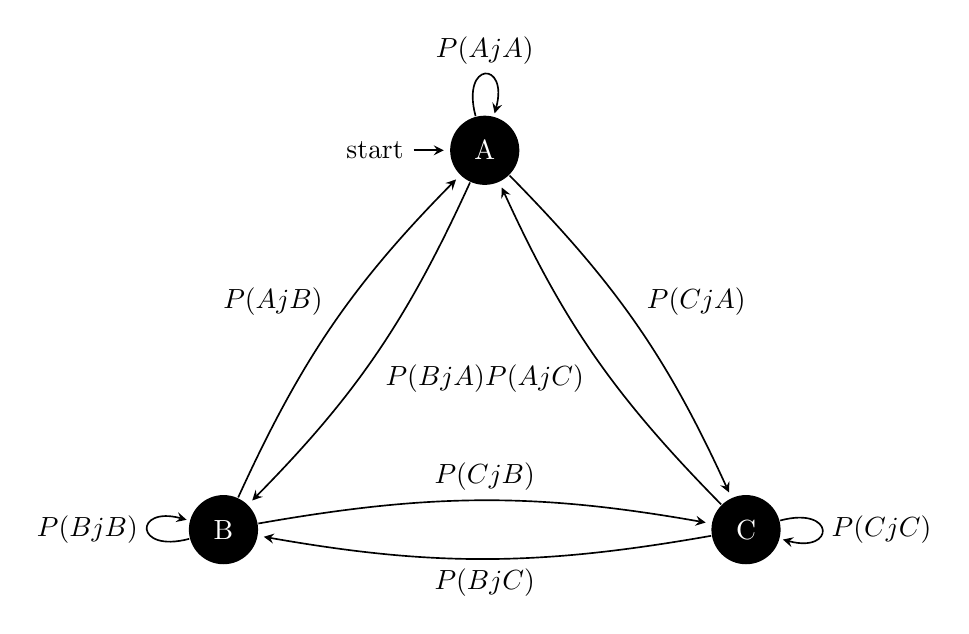
\begin{tikzpicture}[->,>=stealth,shorten >=2pt,auto,node distance=5cm,
semithick]

\tikzstyle{every state}=[fill=black,draw=none,text=white]

\node[initial, state]         (A)                    {A};
\node[state]                  (B) [below left=4.5cm and 3cm]  {B};
\node[state]                  (C) [below right=4.5cm and 3cm] {C};

\path (A) edge [loop above] node {${P(A\textbar A)}$} (A)
          edge [bend left=10] node {${P(B\textbar A)}$} (B)                    
          edge [bend left=10] node {${P(C\textbar A)}$} (C)
      (B) edge [loop left]  node {${P(B\textbar B)}$} (B)
          edge [bend left=10] node {${P(C\textbar B)}$} (C)
          edge [bend left=10] node {${P(A\textbar B)}$} (A)
      (C) edge [loop right] node {${P(C\textbar C)}$} (C)
          edge [bend left=10] node {${P(A\textbar C)}$} (A)
          edge [bend left=10] node {${P(B\textbar C)}$} (B);
\end{tikzpicture}
\note{
Markov Chains are mathematical systems that hop from one "state" (a situation or set of values) to another. That is to say, Markov chains tell you the probability to transition between states in a system. \\
So what takes us from state A to (lets say) state C is a series of jumps relying on probability. \\
}
\end{frame}
\begin{frame}
We can build a transition matrix, $P$, which will then be used to describe the probability for any initial state, $\mu$, to go to a final state, $\nu$. 

\[
P = 
\begin{bmatrix}
	P_{11} & P_{12} & P_{13} &    \dots    & P_{1m} \\
	P_{21} & P_{22} & P_{23} &    \dots    & P_{2m} \\
	\vdots & \vdots & \vdots & P_{\mu \nu} & \vdots \\
	P_{n1} & P_{n2} & P_{n3} &    \dots    & P_{nm}
\end{bmatrix}\vspace{.25cm}\]
For physical systems, we require P to be irreducible and positive recurrent to ensure we "produce" the desired invariant distribution $\pi_\mu$. This stationary distribution has the following properties:
\begin{equation}
\pi = \pi P
\end{equation}
\begin{equation}
\pi_\mu P_{\mu\nu}= \pi_\nu P_{\nu\mu}
\end{equation}
\begin{center}
	Where are our distributions?\\
	Thermodynamical system $ \rightarrow $ Boltzmann Statistics
\end{center}


\note{
As we can see, we only have $\mu \rightarrow \nu$ transitions. That means that Markov chains are "memoryless" or that going to a state only relies on the state you are currently on and not any other step before that. 

4. pi is a row vector in this notation. 

5. definition of detailed balance

\begin{description}
	\item[Irreducibility:] Every state can be reached from any other state in a final number of steps.
	\item[Positive Recurrent:] The chain returns to $\mu$ from $\mu$ in a finite time
\end{description}
}
\end{frame}
\subsection{Metropolis Algorithm}
\begin{frame}
\frametitle{Monte Carlo}
\framesubtitle{Metropolis Algorithm}
Since we know our selection probabilities, $P_{\mu\nu}$ and $ \pi $, we can now move on to making an accept-reject algorithm.\\
If we are on state $ X_n $ and want to test if we will transition to $ Y $, we will do so with the following accept probability

\begin{equation}
X_{n+1} = 
	\begin{cases}
		Y & \rho(X_n,Y_n) \\
		X_n & 1-\rho(X_n,Y_n)
	\end{cases}
\end{equation}

\begin{multline}
	\rho(X_n,Y_n) = 
	min\bigg\{\frac{\pi_Y}{\pi_X}\frac{P_Y}{P_X},1\bigg\} =
	\frac{\pi_Y}{\pi_X}\frac{P_Y}{P_X} = 
	\frac{\frac{1}{Z}e^{-\frac{\mathcal{H}_Y}{k_B T}}}{\frac{1}{Z}e^{-\frac{\mathcal{H}_X}{k_B T}}} =
	e^{-\frac{\mathcal{H}_Y - \mathcal{H}_X}{k_B T}}
\end{multline}

\note{
7. shows our acceptance/flip probability. 

all thats left is just to apply all this in an algorithm. 
}
\end{frame}
\begin{frame}
\begin{enumerate}
	\item Generate a lattice (hot, cold or random)
	\item Pick a point
	\item Test energy
	\item If flipping benefits the lattice, then flip
	\item Otherwise test against $\rho$ with RGN
	\item Repeat
\end{enumerate}
\end{frame}
\section{Results}
\subsection{Metropolis}
\begin{frame}
\frametitle{Results}
\framesubtitle{Metropolis}
Get
\end{frame}

\subsection{Clustering}
\begin{frame}
	content...
\end{frame}




\end{document}